% generated by src/r2/paper_assets (make_paper_assets.py figures); do not edit by hand
% provenance: fig3_robustness generated by src/r2/paper_assets on 2026-10-15 04:07 from data/r2/tables/
%   rob_method_ranking.csv (modified 2026-10-14 19:32): tissue = all_tissues, metric = f1, subset in {all, no_fhb_mode_switch (post hoc)}; lineage: subset = excl_uninformative (post hoc; the configurations in which Family-HB is identified, the same for every estimator); source-clustered intervals mean_D_cluster_lo/hi
%   rob_edge_stability.csv (modified 2026-10-14 19:32): protocol = source, subset = all; jaccard_bfdr_mean and jaccard_top_sizematched_mean (post hoc) with bootstrap intervals over configurations
%   rob_estimator_contrasts.csv (modified 2026-10-14 19:32): reference = family_hb, subset = all, scope = all_tissues (D_f1) or universe (jaccard_bfdr)
%   (constants): bfdr_strong from r2.common.PRESPECIFIED
\begin{figure}[tbp]
  \centering
  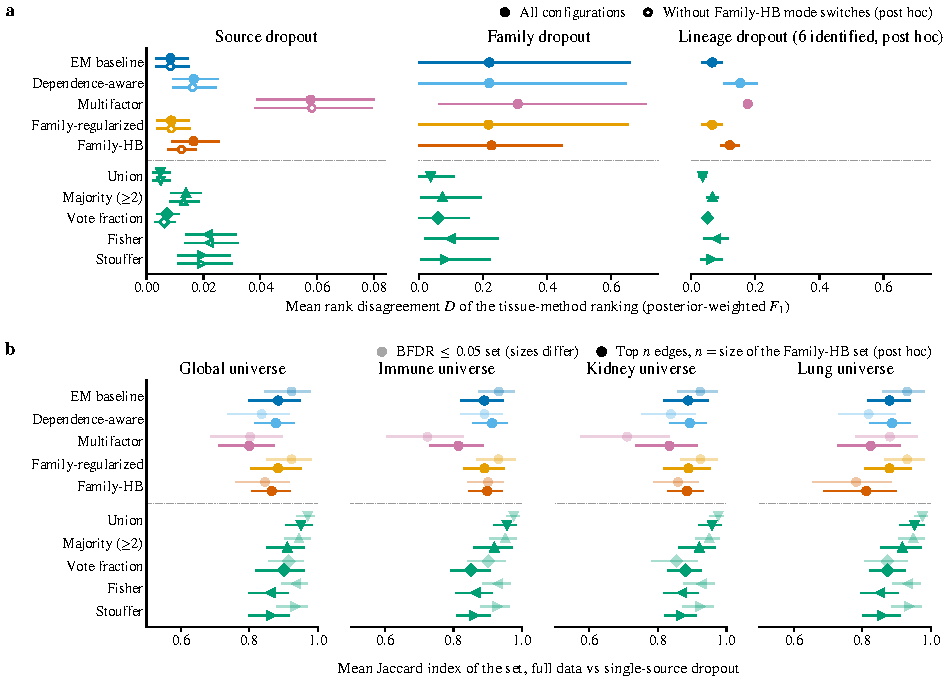
\includegraphics[width=\textwidth]{fig3_robustness.pdf}
  \caption{\textbf{Robustness to annotator dropout.} (a) Mean rank disagreement $D$ \eqref{eq:rankdisagreement} between the method ranking under the full-data credibility and under dropout of one source, one modality family or one integrator lineage, pooled over the three tissue universes (63 source, 9 family and 6 lineage configurations), with 95\% bootstrap intervals clustered by the dropped source, family or lineage (post hoc); family and lineage intervals are descriptive (at most three configurations per universe). Source dropout: Family-HB 0.017 [0.009, 0.025], EM 0.008 [0.003, 0.015], union 0.005 [0.002, 0.009]; open markers (post hoc): the 61 configurations left after removing the 2 in which Family-HB switches posterior mode (lung, SIGNOR and TRRUST dropped), Family-HB 0.012 [0.007, 0.017], EM 0.008 [0.003, 0.015]. Lineage dropout (post hoc): the 6 configurations in which Family-HB is identified, for every estimator (dropping the DoRothEA lineage leaves one modality family, so Family-HB is not identified in 3 of the 9 lineage configurations; post hoc identification rule): Family-HB 0.120 [0.090, 0.151], EM 0.065 [0.032, 0.098]; Family-HB switches posterior mode in 4 of them. (b) Mean Jaccard index between the full-data and the single-source dropout sets (faded markers: BFDR $\leq 0.05$ set; filled markers (post hoc): top $n$ edges, $n$ the size of the Family-HB set), with 95\% bootstrap intervals over the dropout configurations (one per source). For a 0/1 rule the BFDR set is its set of positives, several times larger than the Family-HB set (global universe: Family-HB 4{,}064, EM 18{,}873, union 43{,}444 edges), which inflates its Jaccard index. Global universe, BFDR set: Family-HB 0.85 [0.76, 0.92], EM 0.92 [0.85, 0.98], union 0.97 [0.94, 0.99]; size-matched: Family-HB 0.87 [0.81, 0.92], EM 0.88 [0.80, 0.95], union 0.95 [0.91, 0.98]. The Family-HB values of the lung universe include the source configurations in which Family-HB switches posterior mode (lung, SIGNOR and TRRUST dropped; size-matched Family-HB lung 0.81 [0.69, 0.90]).}
  \label{fig:robustness}
\end{figure}
